The main goal of the simulation experiments was to verify the functionality of the algorithm design. The second goal was to improve the algorithm and its nodes. The third goal was to create several scenarios for the algorithm to test its behavior in different situations. These scenarios were created with later real-world experiments in mind.\\

\section{Algorithm functionality experiments}
    The first experiments were created to test the execution capabilities of the algorithm. They aimed to test if the nodes would not crash or stall the system. These experiments helped to find and fix multiple bugs in the nodes.\\
    Moreover, we were able to detect some weak spots in the BT structure and improve it. The \texttt{Groot} application's log viewer was an invaluable tool for detecting these weak spots. The screen of the log viewer is shown in \ref{fig:log_viewer}.\\
    \begin{figure}[ht]
        \centering
        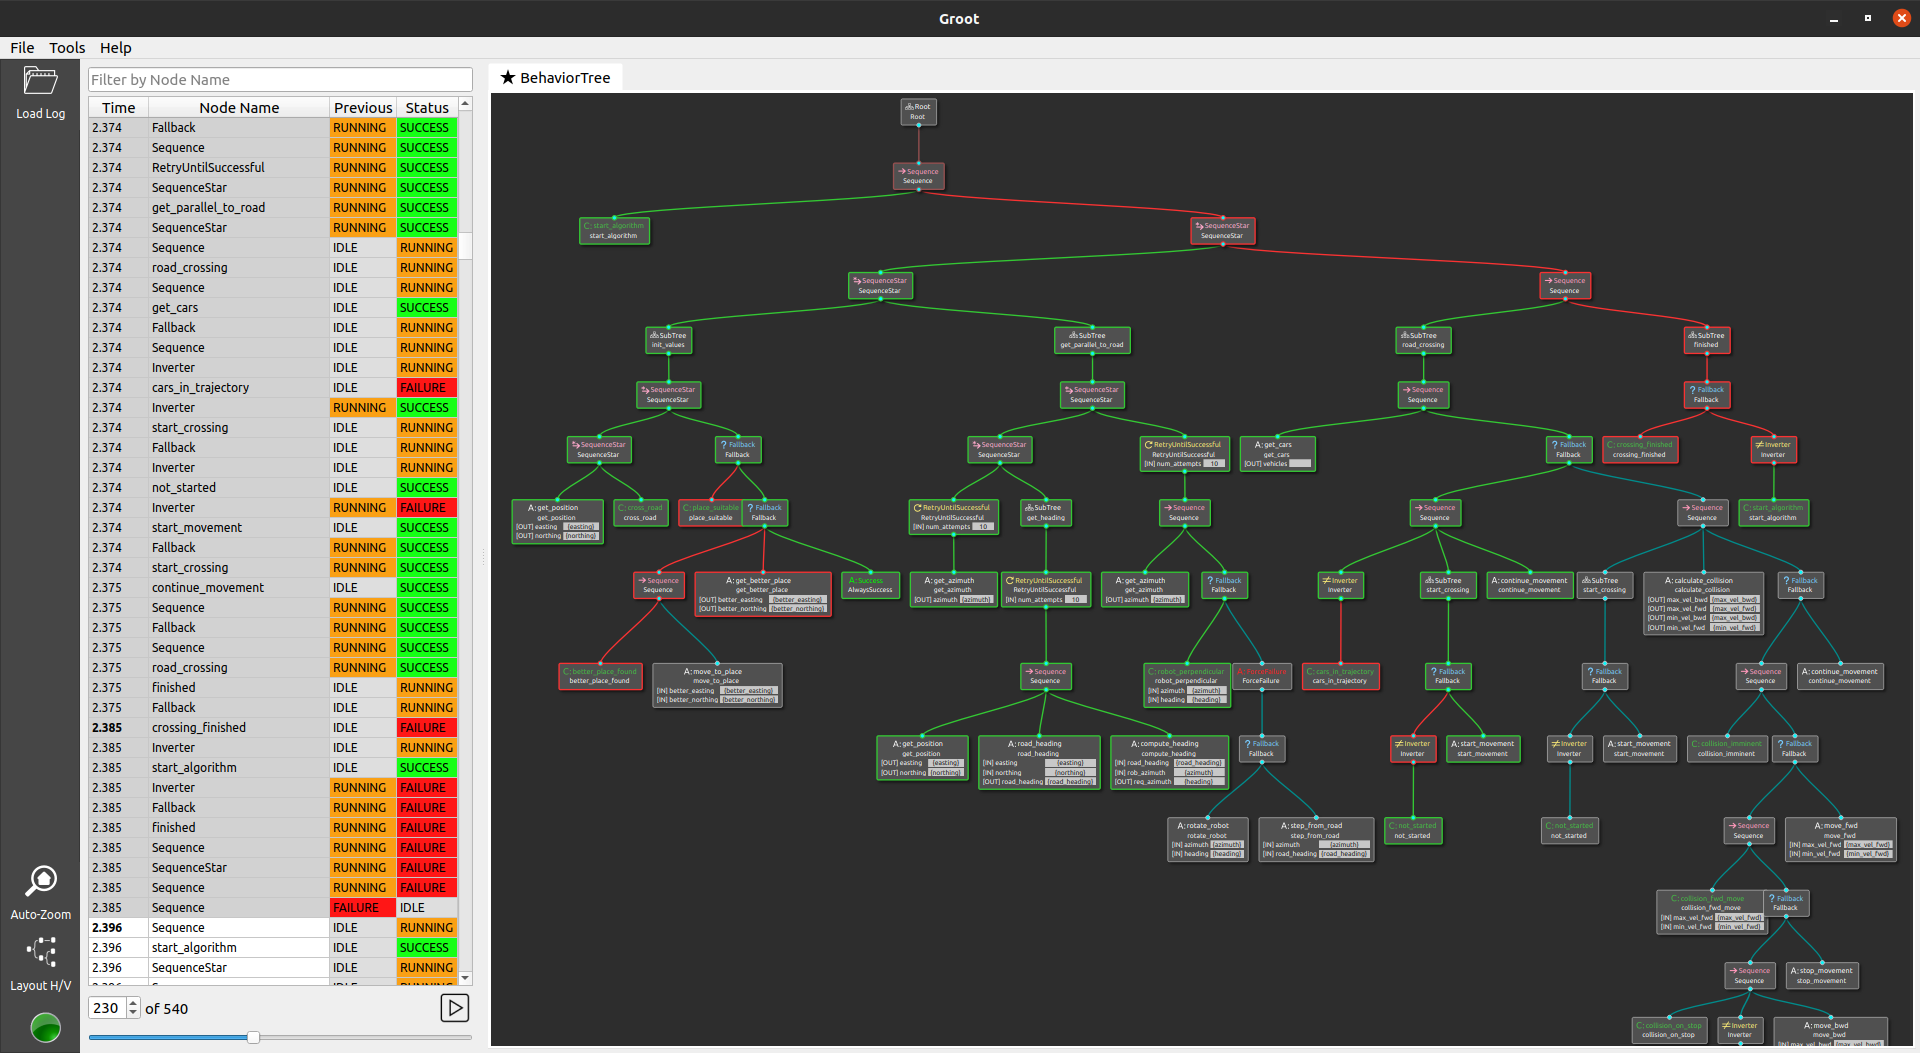
\includegraphics[width=\linewidth]{images/log_viewer.png}
        \caption{Log viewer in \texttt{Groot} application.}
        \label{fig:log_viewer}
    \end{figure}

\section{Algorithm behavior experiments}
    Once the basic functionality was verified, we created several scenarios to test the behavior and universality of the algorithm. This was done to verify that the algorithm would work in different situations.\\
